%  report.tex
%  Document created by seblovett on seblovett-Ubuntu
%  Date created: Tue 01 Apr 2014 19:44:08 BST
%  <+Last Edited: Fri 04 Apr 2014 16:42:18 BST by hl13g10 on octopus +>

\documentclass[12pt]{article}

\usepackage[nodayofweek]{datetime}
\usepackage{graphicx}
\usepackage{todonotes}
\usepackage{multirow} 
\usepackage{listings}
\usepackage{amsmath}
\usepackage{color}
\usepackage{booktabs}
\author{Henry Lovett \\ hl13g10 \\ MEng Electronic Engineering \\ Tutor: Prof. Mark Zwolinski}

\title{ELEC6016 - FPGA Synthesis of a picoMIPS}

%TC:macro \todo 1
\begin{document}
\maketitle
\listoftodos
\begin{abstract}
%\todo[inline]{Abstract: Summarise your work in less than 100 words stating briefly what was achieved.}
This report documents the design and test of a picoMIPS processor.
The processor is able to calculate an affine transform with predefined constants. 
A small instruction set of ten instructions was implemented with an eight bit opcode format. 
The processor is a register-accumulator based architecture. 
\end{abstract}
%TC:ignore



\definecolor{mygreen}{rgb}{0,0.6,0}
\definecolor{mygray}{rgb}{0.5,0.5,0.5}
\definecolor{mymauve}{rgb}{0.58,0,0.82}

%Code Styles
\lstset{basicstyle=\scriptsize\ttfamily,
  backgroundcolor=\color{white},   % choose the background color; you must add \usepackage{color} or \usepackage{xcolor}
  basicstyle=\footnotesize,        % the size of the fonts that are used for the code
  breakatwhitespace=false,         % sets if automatic breaks should only happen at whitespace
  breaklines=true,                 % sets automatic line breaking
  captionpos=t,                    % sets the caption-position to bottom
  commentstyle=\color{mygreen},    % comment style
  deletekeywords={...},            % if you want to delete keywords from the given language
  escapeinside={\%*}{*)},          % if you want to add LaTeX within your code
  extendedchars=true,              % lets you use non-ASCII characters; for 8-bits encodings only, does not work with UTF-8
  frame=single,                    % adds a frame around the code
  keepspaces=true,                 % keeps spaces in text, useful for keeping indentation of code (possibly needs columns=flexible)
  numbers=left,                    % where to put the line-numbers; possible values are (none, left, right)
  numbersep=5pt,                   % how far the line-numbers are from the code
  numberstyle=\tiny\color{mygray}, % the style that is used for the line-numbers
  rulecolor=\color{black},         % if not set, the frame-color may be changed on line-breaks within not-black text (e.g. comments (green here))
  showspaces=false,                % show spaces everywhere adding particular underscores; it overrides 'showstringspaces'
  showstringspaces=false,          % underline spaces within strings only
  showtabs=false,                  % show tabs within strings adding particular underscores
  stepnumber=1,                    % the step between two line-numbers. If it's 1, each line will be numbered
  tabsize=2,                       % sets default tabsize to 2 spaces
  title=\lstname                   % show the filename of files included with \lstinputlisting; also try caption instead of title
}
\lstdefinestyle{sverilog} {
  language=Verilog,
  otherkeywords={always\_ff,always\_comb,assert,logic,return,\$random,\#*},            % if you want to add more keywords to the set
  stringstyle=\color{mymauve},     % string literal style
  keywordstyle=\color{blue}      % keyword style
}
\lstdefinestyle{asm} {
  otherkeywords={PASSA,MULT,ADD,STACC,LUI,ADDI,STSW,WAIT0,WAIT1,JMPA},            % if you want to add more keywords to the set
  keywordstyle=\color{blue},       % keyword style
  language={[x86masm]Assembler}                % the language of the code
}

\todo[inline]{Get \# numbers coloured in verilog listings}
%\todo[inline]{Neaten all synthesis figures}
%\todo[inline]{Standardise all tables}
\todo[inline]{Spell Check}

%TC:endignore
%For each:
% Design of
% Test
%  Introduction.tex
%  Document created by seblovett on seblovett-Ubuntu
%  Date created: Tue 01 Apr 2014 19:50:43 BST
%  <+Last Edited: Sat 26 Apr 2014 11:54:41 BST by hl13g10 on octopus +>

\section{Introduction}\label{sect:intro}
%\todo[inline]{Introduction to do}
%State the objectives of the assignment. Summarise briefly your preparation work,  your experimental work,, and results achieved. Specifically, state which parts of the assignment were delivered according to the requirements and summarise any extensions to the basic specification you have carried out with references to the sections.  ( approx. 0.5 page).

This assignment is to design and test a processor capable of executing an affine transform of a vector. 
The processor should be optimised in terms of size, with no performance requirements. 
The cost function, seen in equation~\eqref{eq:cost}, should be minimised. 
The data is given in bytes and must be read from the switches and the result should be displayed on the LEDs. 
A handshaking protocol is also defined and must be followed. 
A processor is defined as having a distinct control, datapath and memory with an instruction set that is executed. 

\begin{equation}\label{eq:cost}
\mbox{Cost} = \mbox{ Number of Logic Elements} + 30 \times \mbox{Kbits of RAM}
\end{equation}

A number of designs and approaches were investigated, including register-register and single cycle designs.
The final design is a register-accumulator, multi-cycle processor which utilises embedded multipliers and SRAM available on the target FPGA. 
It is able to conduct the affine transform using data set 2, shown in equation \eqref{eq:affinedata2}, and satisfies the handshaking protocols. 

\begin{equation}\label{eq:affinedata2}
\begin{bmatrix}
x_2 \\
y_2 
\end{bmatrix}
=
\begin{bmatrix}
0.5 & -0.875 \\
-0.875 & 0.75 
\end{bmatrix}
\begin{bmatrix}
x_1 \\
y_1
\end{bmatrix}
+
\begin{bmatrix}
5 \\
12
\end{bmatrix}
\end{equation}


Figure \ref{fig:arch} shows the architecture of the processor, excluding the control and control signals.

\begin{figure}
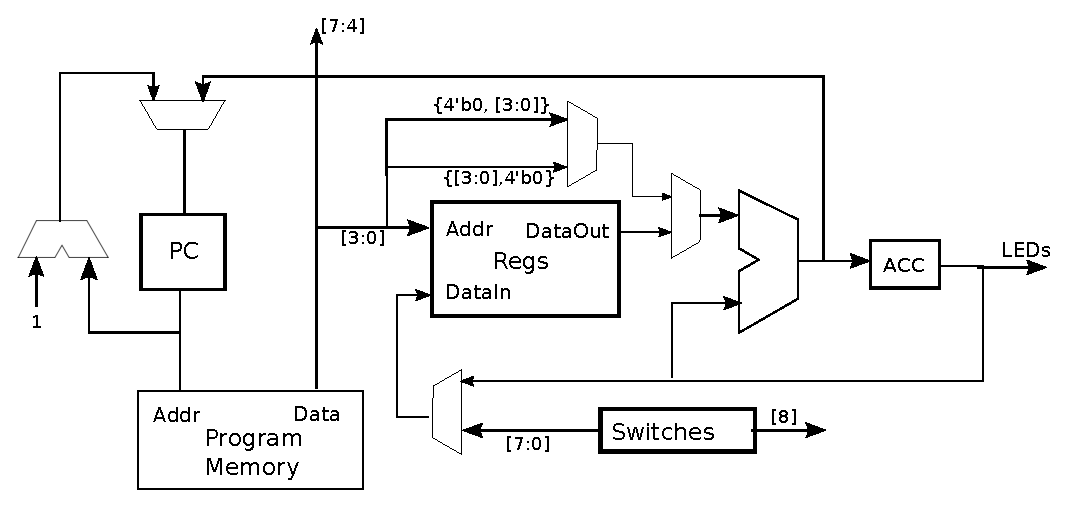
\includegraphics[width=\textwidth]{Figures/architecture.eps}
\caption{Block Diagram of the architecture. Control unit and signals have been omitted for clarity.}
\label{fig:arch}
\end{figure}

Each module of the processor is documented in this report, with discussion on the design, test and synthesis of the code. 
Additional extras are also discussed, including a simple assembler (see Section \ref{sect:prog} and extra logic added for debugging and the demonstration (see Section \ref{sect:de0}.

%  Architecture.tex
%  Document created by seblovett on octopus
%  Date created: Wed 02 Apr 2014 14:03:33 BST
%  <+Last Edited: Wed 02 Apr 2014 14:47:11 BST by hl13g10 on octopus +>

\section{Architecture}

Discuss the overall architecture

A register-accumulator based architecture was decided to be used. 
This results in the instruction only needing one operand, reducing the overall size. 
Figure \ref{fig:arch} shows the architecture of the processor, excluding the control and control signals.

\begin{figure}
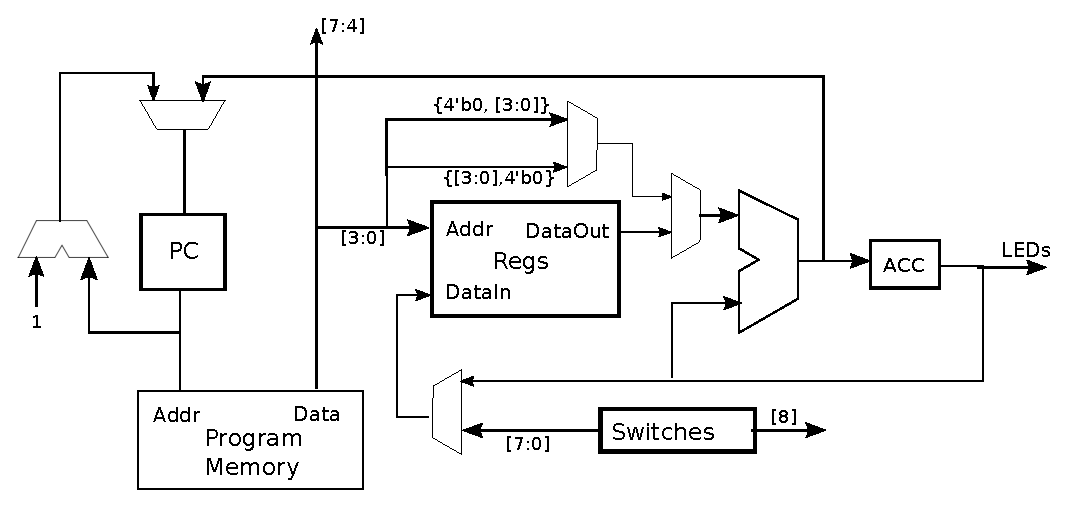
\includegraphics[width=\textwidth]{Figures/architecture.eps}
\caption{Block Diagram of the architecture. Control unit and signals have been omitted for clarity.}
\label{fig:arch}
\end{figure}

Each aspect of the processor are discussed in the following sections, looking at the design, test and synthesis of the modules.

% ISA.tex
%  Document created by seblovett on seblovett-Ubuntu
%  Date created: Tue 01 Apr 2014 20:08:47 BST
%  <+Last Edited: Sat 26 Apr 2014 11:56:13 BST by hl13g10 on octopus +>


\section{Instruction Set}

%Discuss what instructions are implemented
In total, ten instructions are implemented in the design.
They are fully documented in table \ref{tab:isa}. 


\begin{table}
\caption{Instruction Set and their operations}
\label{tab:isa}
\begin{tabular}{ccc} \toprule
Instruction & Acronym & Operation \\ \midrule
Store Switches & STSW Rn & Rn $\leftarrow$ Switches[7:0] \\
Store Accumulator & STACC Rn & Rn $\leftarrow$ Acc \\
Wait while 0 & WAIT0 & if(Switches[8] == 1) Pc++ \\
Wait while 1 & WAIT1 & if(Switches[8] == 0) Pc++ \\
Absolute Jump & JMPA Imm & PC $\leftarrow$ Acc + Imm \\
Load Upper Immediate & LUI Imm & Acc $\leftarrow$ {Imm, 4'b0000} \\
Add Immediate & ADDI Imm & Acc $\leftarrow$ Acc + Imm \\
Add Register & ADD Rn & Acc $\leftarrow$ Acc + Rn \\
Multiply Register & MULT Rn & Acc $\leftarrow$ Acc * Rn \\
Pass Register & PASSA Rn & Acc $\leftarrow$ Rn \\ \bottomrule
\end{tabular}
\end{table}


\subsection{Arithmetic Instructions}

Only three instructions implemented conduct arithmetic operations, \texttt{ADD}, \texttt{ADDI} and \texttt{MULT}. 
These are all signed arithmetic and are the only functions needed to compute the affine transform. 
Add immediate (\texttt{ADDI}) is the addition of a four bit unsigned immediate. 
No subtract immediate instruction was implemented to reduce the size of the ALU and no sign extension is needed for the immediate. 

\subsection{Accumulator and Register Instructions}
%LUI, STSW, STACC, PASSA

The switches provide the main data input to the processor. 
A store switches instruction (\texttt{STSW}) is implemented to directly store to a register. 
Load upper immediate (\texttt{LUI}) is used to load constants from the program memory to the accumulator. 
Used in conjunction with the \texttt{ADDI} instruction, any 8 bit value can be loaded to the accumulator in two instructions. 
This can then be used to make a negative number to use for an arithmetic function.

The register-accumulator design, although allows for only one operand in the instruction, must also include extra instructions to move data.
The instructions needed are a pass to accumulator (\texttt{PASSA}), to write a value from a register to the accumulator, with no modification. 
A store accumulator instruction (\texttt{STACC}) is also needed to write back the data to a register. 

\subsection{Control Instructions}

The affine transform does not involve any decisions based on the data. 
The only required control flow is during the handshaking protocol. 
As this is reliant on the value of Switches[8], this is accomplished by two instructions, \texttt{WAIT0} and \texttt{WAIT1}. 
These will only allow the program counter to increment if the value of Switches[8] is correct.
This means no flags need to be used in the design, and no conditional branches. 

An absolute jump instruction is also implemented (\texttt{JMPA}). 
It is used once the affine transform is complete to return to the start of the loop.
This replaces the value of the program counter with what is stored in the accumulator plus a four bit immediate. 
It means that the processor can jump to any eight bit memory location in two instructions.


\subsection{Instruction Format}

A total of ten instructions have been implemented. 
The ten instructions and the use of a four bit immediate, lends the instruction set to use an eight bit instruction format.
This is summarised in table \ref{tab:instruction}.
A simple instruction format lends itself to simple decoding. 
A maximum of sixteen general purpose registers (assuming no dummy register) can be used.

\begin{table}[b]
\caption{The instruction format used}
\label{tab:instruction}
\centering
\begin{tabular}{|p{1cm}|p{1cm}|p{1cm}|p{1cm}|p{1cm}|p{1cm}|p{1cm}|p{1cm}|p{1cm}|} \hline
Bit & 7 & 6 & 5 & 4 & 3 & 2 & 1 & 0 \\ \hline
Use & \multicolumn{4}{|c|}{Opcode} & \multicolumn{4}{|c|}{Immediate / Register} \\ \hline
\end{tabular}
\end{table}

%  Controller.tex
%  Document created by seblovett on seblovett-Ubuntu
%  Date created: Tue 01 Apr 2014 20:09:16 BST
%  <+Last Edited: Sat 26 Apr 2014 11:58:08 BST by hl13g10 on octopus +>


\section{Controller}\label{sect:controller}

The controller is the decoding sequential logic of a processor. 
It decodes the opcode into the correct signals for the multiplexers, ALU operations and enable signals.


\subsection{Design}

%why a multicyclsis needed
The controller used is sequential. 
This is due to the program memory and registers being sequential memory (see sections \ref{sect:prog} and \ref{sect:regs}).
Three states are implemented, \texttt{Fetch}. \texttt{Read} and \texttt{Execute}. 
During the \texttt{Fetch} cycle, the program memory is accessed with a new address. 
This then stores the instruction at the output of the program memory. 
\texttt{Read} is needed to allow the read of the registers. 
By the \texttt{Execute} cycle, both the register value and the instruction are available. 
Any instruction can then be conducted at this point.
Some instructions (\texttt{LUI}, \texttt{STSW}, \texttt{WAIT0}, \texttt{WAIT1}, \texttt{JMPA}, \texttt{STACC}) do not necessarily need three cycles to complete as the do not use a register value.
However, keeping all instructions to execute in the same number of cycles reduces the complexity of the decoder. 
Figure \ref{fig:controllerasm} shows the state transition diagram generated by the Quartus synthesis tool.

\begin{figure}
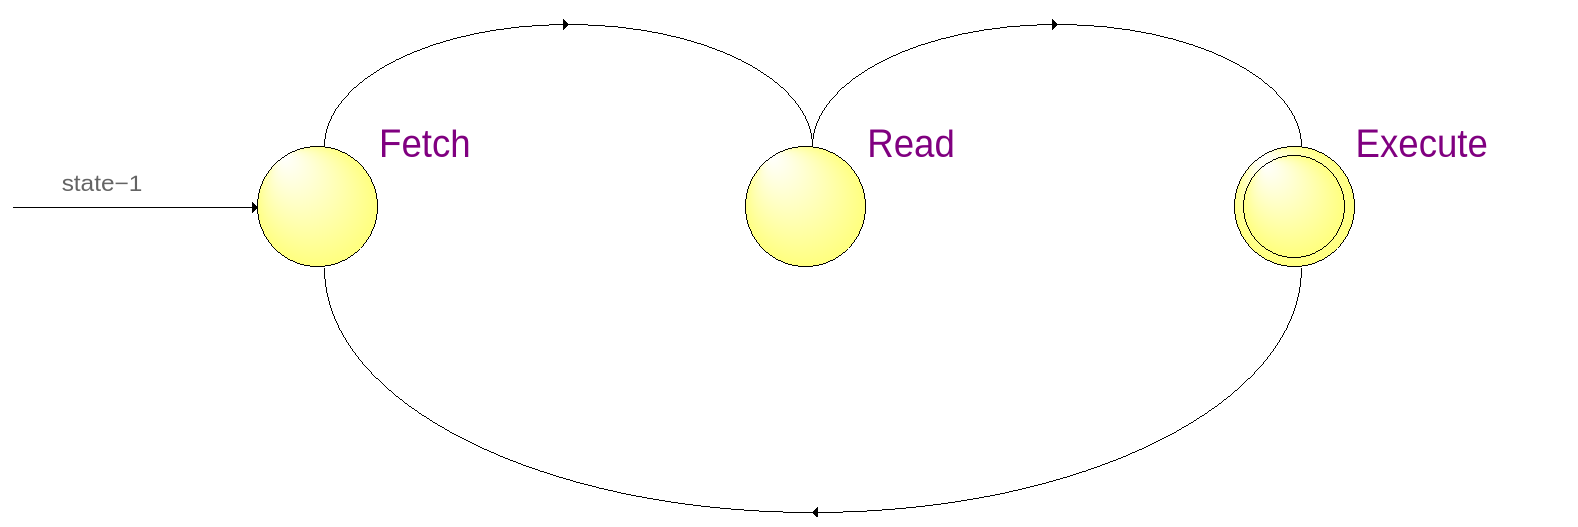
\includegraphics[width=\textwidth]{Figures/cpu_control_state.png}
\caption{State transition diagram for controller}
\label{fig:controllerasm}
\end{figure}

%Opcode assignments to the instruction set
By careful allocation of the opcode values, the controller can be greatly simplified. 
Each of the instructions in table \ref{tab:isa} must have a unique four bit value. 
There are eight control signals for the ALU operation, multiplexer selection or write enable for a register. 
The combinational control signals do not rely on the state, and so can be reduced to a function between the bits of the opcode. 
The sequential control signals, however, must only be asserted during one cycle of an instruction and are therefore dependent on the state. 

Table \ref{tab:controlsignals} shows all the control signals between the datapath and the controller. 
All signals default to 0.
The instructions which assert the signals are listed in table \ref{tab:controlsignals}. 
By grouping these instructions together, the control signals can then be reduced to simple logic operations.
The assignment of opcodes to the instructions is seen in table \ref{tab:kmap}. 
The most simple optimisation done is allowing the bottom two bits of the instruction to be the ALU operation. 
In this case, 0 will be a pass through instruction, 1 will be an add and 3 will be a multiply. 
As 2 is not used by any instruction, this can be set to anything in the ALU.
This removes all need for any logic to decode the ALU function. 

For the \textit{ImmSel} signal, it requires more logic. 
Table \ref{tab:kmap:immsel} shows a K-Map for the \textit{ImmSel} signal, replacing the instructions with values.
A lot of instructions are not affected by this control signal as it only affects the instructions using the immediate. 
This results in a very simple logic expression of $!(Opcode[0] | Opcode[1])$, i.e. the \texttt{NOR} between the lowest two bits of the opcode. 
This can be done for all the signals, except \textit{PcWe} as this is reliant on the value for of \textit{Switches[8]}. 
The sequential signals can be minimised in a similar fashion, but are only asserted in the execute state.
Listing \ref{controlopt} shows all the signals with their reduced decoding. 

\begin{table}
\caption{Control signals and the instructions where they are asserted (are logic 1)}
\label{tab:controlsignals}
\centering
\begin{tabular}{ccc} \toprule
Type & Signal Name & Instruction(s) \\ \midrule
\multirow{5}{*}{Combinational} & PcSel & JMPA \\ 
 & ImmSel & LUI \\
 & Op1Sel & JMPA, LUI, ADDI \\
 & WDataSel & STSW \\ 
 & AluOp & LUI, JMPA, PASSA, ADD, ADDI, MULT \\ \midrule
\multirow{3}{*}{Sequential} & PcWe & WAIT0 WAIT1 \\
 & RegWe & STSW, STACC \\
 & AccWe &  PASSA, ADD, ADDI, MULT, LUI \\ \bottomrule

\end{tabular}
\end{table}

%\todo[inline]{K maps to show the minimized logic}


\begin{table}
\caption{Opcode allocation to the instructions}
\label{tab:kmap}
\centering
\begin{tabular}{|c|c|p{1.5cm}p{1.5cm}p{1.5cm}p{1.5cm}|}\cline{3-6}
\multicolumn{2}{c|}{} & \multicolumn{4}{|c|}{Opcode[3:2]} \\ \cline{3-6}
\multicolumn{2}{c|}{} 			& 00	& 01	& 11	& 10	\\  \hline
\multirow{4}{*}{Opcode[1:0]} 	& 00 	& STSW	& -	& PASSA	& LUI	\\
				& 01 	& STACC	& JMPA	& ADD	& ADDI	\\
				& 11 	& WAIT0	& WAIT1	& MULT	& -	\\
				& 10 	& -	& -	& -	& -	\\ \hline

\end{tabular}
\end{table}

\begin{table}
\caption{K-map of the \textit{ImmSel} Control Signal - X is don't care}
\label{tab:kmap:immsel}
\centering
\begin{tabular}{|c|c|p{1.5cm}p{1.5cm}p{1.5cm}p{1.5cm}|}\cline{3-6}
\multicolumn{2}{c|}{} & \multicolumn{4}{|c|}{Opcode[3:2]} \\ \cline{3-6}
\multicolumn{2}{c|}{} 			& 00	& 01	& 11	& 10	\\  \hline
\multirow{4}{*}{Opcode[1:0]} 	& 00 	& X	& X	& X	& 1	\\
				& 01 	& X	& X	& X	& 0	\\
				& 11 	& X	& 0 	& X	& X	\\
				& 10 	& X	& X	& X	& X	\\ \hline

\end{tabular}
\end{table}

\lstinputlisting[style=sverilog, firstline=40, lastline=54,caption={Reduced Control signal allocations},label=controlopt]{../Implementation/control.sv}



%\todo[inline]{Neaten State transition diagram}
%\todo[inline]{Testbench}
\subsection{Testbench}

To test the controller, each instruction was passed in turn.
During the execute cycle of the controller, the relevant outputs are checked. 
Assertions are used to verify the expected behaviour. 
If an assertion fails, an error counter is incremented. 
By the end of the simulation, the error counter should be zero.
Figure \ref{fig:controllersim} shows the waveform of the simulation.
%Each opcode is tested in turn.
All inputs and outputs are shown, along with the internal state of the controller and the error counter.
The error counter is at zero at the end of the simulation, showing that this testbench passes. 

\begin{figure}
\includegraphics[height=\textheight-1cm]{Figures/controllersim.eps}
\caption{Controller simulation waveform}
\label{fig:controllersim}
\end{figure}


\subsection{Synthesis}

%\todo[inline]{Synthesis}

The synthesis of the controller is seen in figure \ref{fig:control:synth}.
The largest part of the controller is the state machine. 
All of the discussed simplifications to the decoding can be seen in this diagram.
Interestingly, the dependence of the write enable signals is realised by a multiplexer.
A simpler solution could be an \texttt{AND} gate. 
If the state is encoded using one hot coding, then no extra logic would be required to use an \texttt{AND} gate.
However, the synthesis tool probably takes into account the layout of the device and utilises the logic blocks as much as possible.


\begin{figure}
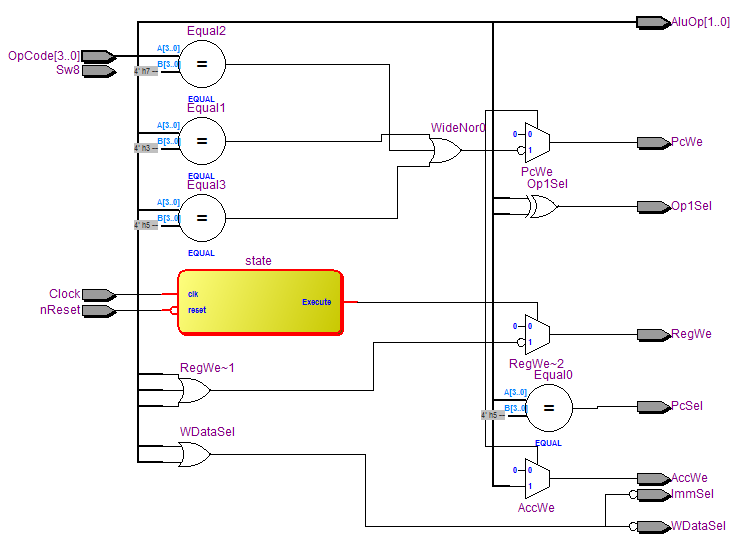
\includegraphics[width=\textwidth]{Figures/controlsynth.png}
\caption{Synthesis of the controller}
\label{fig:control:synth}
\end{figure}



%  Program.tex
%  Document created by seblovett on seblovett-Ubuntu
%  Date created: Tue 01 Apr 2014 20:09:49 BST
%  <+Last Edited: Sat 26 Apr 2014 12:13:43 BST by hl13g10 on octopus +>

\section{Program}\label{sect:prog}

%\todo[inline]{The program counter, how and why it works}
\subsection{Program Counter}
The program counter is a register storing the address of the current instruction.
It is used to access the program memory to retrieve instructions. 
The implementation involves a six bit write enable register with a multiplexed input. 
The inputs to the multiplexer are the output of the ALU and an incremented value of itself.
The increment is used to progress the program in normal operation, where as the ALU output is used to jump to any location by use of the \texttt{JMPA} instruction.
Only six bits are used as the program implemented is 46 instructions long. 

\subsection{Program Memory}
The program memory is implemented as sequential read only memory (ROM). 
%This means there is no ability to write to the memory.
It takes a clock cycle to output the data at the given address. 
This is advantageous as the Cyclone IV has a large amount of synchronous RAM, which is far more efficient that using logic elements.
However, this then requires a multi-cycle control module. 

%\todo[inline]{Program itself}
\subsection{Program}

The program is in two sections, the set up and the loop. 
The set up loads all the constants into the registers. 
The loop then conducts the handshaking and the affine transform. 

\subsubsection{Set Up}

The initial part of the program loads in the matrix coefficients into the registers. 
The coefficients of the \textbf{A} matrix are represented by fixed point notation. 
This means that the values must be 128 times bigger than the decimal equivalent.
Listing \ref{lstsetupcode} shows the code to load all the constants to memory.

\lstinputlisting[style=asm,lastline=18,caption={Loading initial constants},label=lstsetupcode]{../Implementation/transform.asm}


\subsubsection{Loop}

An initial handshake is done to load the values of $x_1$ and $y_1$ into memory. 
This is achieved by using the \texttt{WAIT}\textit{n} instructions to control the program flow, and the \texttt{STSW} to write the switches to a memory location. 
The whole process is seen in listing \ref{lsthandshake1}.

\lstinputlisting[style=asm,firstline=19, lastline=24,caption={Handshaking protocol for switch reading},label=lsthandshake1]{../Implementation/transform.asm}


The affine transform is shown in equation \eqref{eq:affine}.
By multiplying the matrix out, $x_2$ and $y_2$ can be calculated by equations \eqref{eq:x2} and \eqref{eq:y2} respectively. 
Listing \ref{lstaffinex} shows the instructions used to calculated $x_2$. 
The $y_2$ value is calculated in the same way, using different source registers.

\begin{equation}\label{eq:affine}
\begin{bmatrix}
x_2 \\
y_2 
\end{bmatrix}
=
\begin{bmatrix}
a_{11} & a_{12} \\
a_{21} & a_{22} 
\end{bmatrix}
\begin{bmatrix}
x_1 \\
y_1
\end{bmatrix}
+
\begin{bmatrix}
b_1 \\
b_2
\end{bmatrix}
\end{equation}

\begin{equation}\label{eq:x2}
x_2 = a_{11} \times x_1 + a_{12} \times y_1 + b_1
\end{equation}

\begin{equation}\label{eq:y2}
y_2 = a_{21} \times x_1 + a_{22} \times y_1 + b_2
\end{equation}


\lstinputlisting[firstline=25, lastline=35,caption={Affine transform for calculating $x_2$},label=lstaffinex,style=asm]{../Implementation/transform.asm}


Once the transform is complete, a second handshake is done to read back the result. 
The program then jumps to the start of the loop, ready for the next calculation. 
This code is seen in listing \ref{lsthandshake2}.
\newpage
\lstinputlisting[firstline=41, lastline=46,caption={End of loop code to display results and return to the beginning of the loop},style=asm,label=lsthandshake2]{../Implementation/transform.asm}


%\todo[inline]{Talk about assembler too?}
%\todo[inline]{Jump locations in asm? Be good to implement. Filling all of memory too? If I'm doing this, .defines also... I said it's a simple. Brownie points for doing one full stop, but no need to make my life difficult.}
A basic assembler is implemented to aid development.
It is capable of reading the SystemVerilog package containing the definition of the opcodes.
It then assembles the program into the hex values. 
Concurrent development of programs and processor is then greatly simplified as all definitions are obtained from the same package.
It is written in python and accepts command line arguments to compile a asm file.
A help prompt is also given when \texttt{-h} is given as an argument.


The testing of the program counter is done as a part of the datapath test and is discussed in section \ref{sect:datapath}.
%\todo[inline]{Is it possible to test? It is part of the overall datapath.}
%\todo[inline]{synthesis?}
\subsection{Synthesis}

The synthesised logic of the ROM can be seen in figure \ref{fig:ramsynth}.
It shows that there is some redundancy in the logic as the standard cells contain write circuitry.
Here, constants are used to disable the functionality, as these are fabricated, rather than built out of logic elements.


\begin{figure}
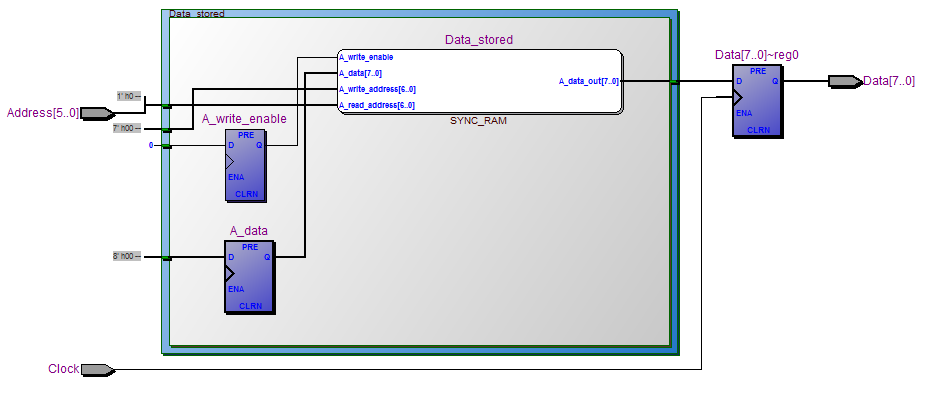
\includegraphics[width=\textwidth]{Figures/ramsynth.png}
\caption{Synthesis of the Program ROM module}
\label{fig:ramsynth}
\end{figure}
% and Program Memory
%\input{Program Counter}
%  Registers.tex
%  Document created by seblovett on seblovett-Ubuntu
%  Date created: Tue 01 Apr 2014 20:10:32 BST
%  <+Last Edited: Fri 04 Apr 2014 10:11:29 BST by hl13g10 on octopus +>

\section{Registers}\label{sect:regs}

%\todo[inline]{Design}
The allocation in the instruction set allows for up to 16 general purpose registers. 
In the program, discussed in section \ref{sect:prog}, only 11 registers are used. 
Six are used to store the constants, two for the initial vector, two for the result and a temporary register.
To save RAM, only the required registers are implemented.
This still requires a four bit address and attempting to address the registers above the valid range would result in undefined behaviour.

The registers were implemented using the Synchronous RAM.
This, at the expense of performance, utilised the on chip SRAM blocks. 
The design was parametrised to allow the data and address width and number of registers to be easily changed. 

%\todo[inline]{Explain Test Bench}

\subsection{Testbench}

A task is used to do a basic test.
The code for this task is seen in listing \ref{lstregtask}.
A random byte of data, and a random register are chosen. 
The data is then written to the register. 
The input data is changed to check that the data on the output is stored in memory and assertions are used to verify. 
The data is checked to persist after the write enable signal is inactive. 
If an assertion fails, a global error counter is incremented.

This task is then done a large amount of times to check all registers. 
Figure \ref{fig:regsim} shows the output waveform of the simulation. 
The error count is zero at the end of the simulation showing that the module is functioning correctly.




\lstinputlisting[language=verilog,breaklines=true, firstline=33, lastline=51,caption={Register task for writing and reading to the register.},frame=single,label=lstregtask]{../Implementation/registers_stim.sv}
%\todo[inline]{Simulation Results}

\begin{figure}
\includegraphics[width=\textwidth,height=\textheight]{Figures/registerssim.eps}
\caption{Waveform simulation for register testbench}
\label{fig:regsim}
\end{figure}

\subsection{Synthesis}
\todo[inline]{Synthesis}

%  ALU.tex
%  Document created by seblovett on seblovett-Ubuntu
%  Date created: Tue 01 Apr 2014 20:10:56 BST
%  <+Last Edited: Fri 04 Apr 2014 12:37:03 BST by hl13g10 on octopus +>


\section{ALU}

\subsection{Design}
The arithmetic logic unit (ALU) is a key part of a processor. 
It is a combinational block of memory, responsible for the arithmetic and logic operations on the data.
The ALU in this processor has three operations on two operands.
No flags, such as carry or zero, are implemented either as no conditional branches are needed.

The ALU supports the operations in table \ref{tab:aluops}.
The operation encodings are discussed in section \ref{sect:controller}.
Due to the use of fixed point notation, the integer result of the multiplication is located at bits [14:7] of the 16 bit result.
To correctly synthesised combinational logic, all inputs must have a defined output.
The ALU was smallest in size when the A function was repeated in the redundant state.

\begin{table}
\caption{ALU Operations supported}
\label{tab:aluops}
\begin{tabular}{|c|c|c|} \hline
Operation & Explanation & Encoding (binary)\\  \hline
A & Result = Operand1 & 00, 10 \\
Add & Result = Operand1 + Operand2 & 01 \\
Multiply & Result = (Operand1 $\times$ Operand2)[14:7] & 11 \\ \hline
\end{tabular}
\end{table}


The Cyclone IV FPGA has a number of embedded multipliers. 
One of these is utilised within the ALU to conduct signed multiplication. 
This is done by defining the inputs as signed, and using a combinational assign statement.
The Quartus tool then recognises this and synthesises the design using the embedded multipliers.
The multiplier cell also includes 3 registers which are not utilised in this design.


%\todo[inline]{Operations implemented}
%\todo[inline]{Embedded multiplier(s)}
%\todo[inline]{Explain Test bench}

\subsection{Testbench}

The testbench tests each operation with ten different values of the operands. 
An assertion then checks each result is as expected. 
An error count is kept and the simulation is successful if this is zero at the end of the simulation.
Figure \ref{fig:alusim} shows the waveform for the simulation. 
It can be seen that all three operations are tested and the error count is zero at the end. 
The fourth, undefined operation is not tested as the result does not matter. 

\begin{figure}
\includegraphics[height=\textheight]{Figures/alusim.eps}
\caption{Simulation waveform for the ALU testbench}
\label{fig:alusim}
\end{figure}

%\todo[inline]{Simulation results}
%\todo[inline]{Synthesis}
\subsection{Synthesis}

Synthesis of the ALU largely consists of multiplexors. 
As three operations are implemented, this requires 8 3:1 multiplexors. 
There is also adder and multiplier. 
The multiplier implemented utilised the embedded multipliers available on the device.

\begin{figure}
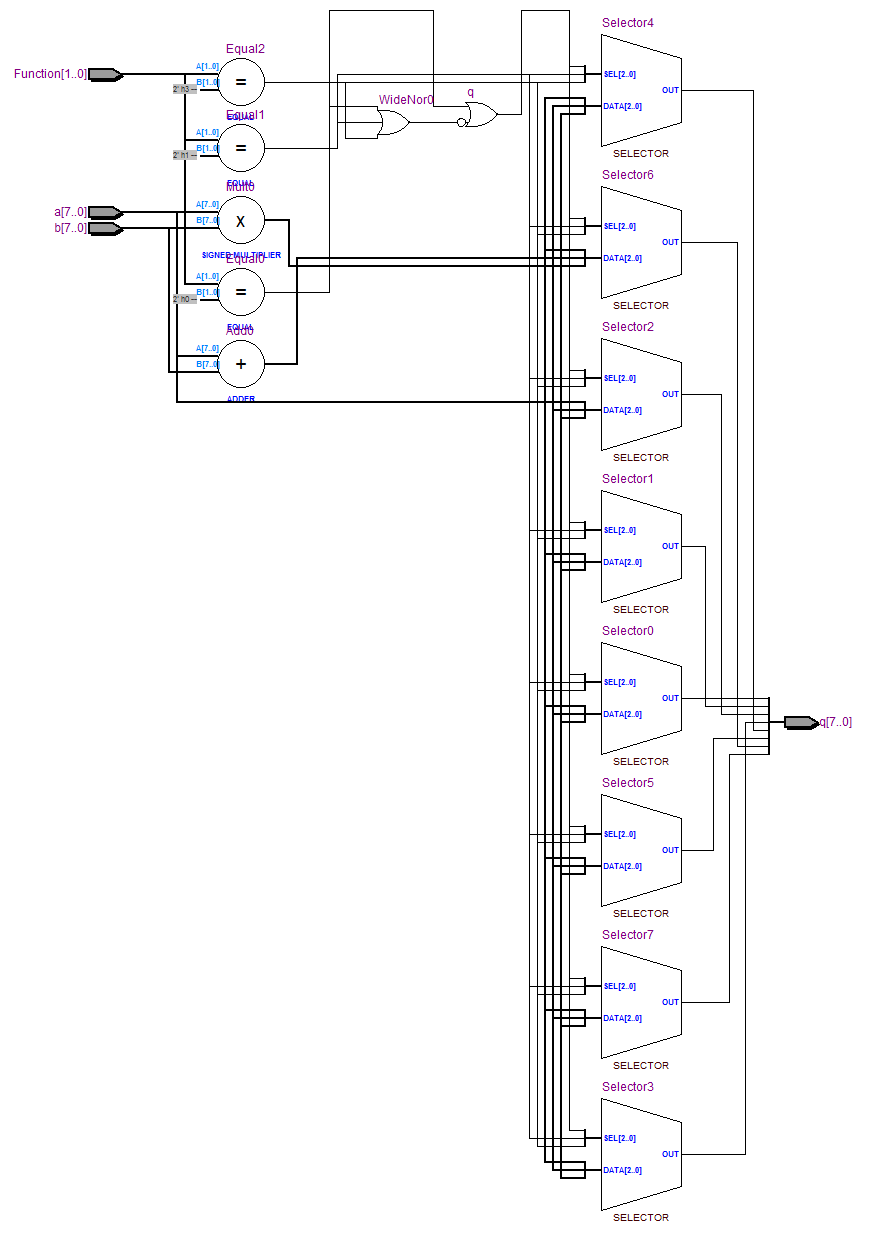
\includegraphics[height=\textheight]{Figures/alusynth.png}
\caption{Synthesis of the Arithmetic Logic Unit}
\label{fig:alusynth}
\end{figure}

%  cpu.tex
%  Document created by seblovett on octopus
%  Date created: Thu 03 Apr 2014 12:56:02 BST
%  <+Last Edited: Fri 04 Apr 2014 15:38:15 BST by hl13g10 on octopus +>

%\section{Processor}

%The whole processor is pulled together in two encapsulating modules. 
%The datapath module links the registers and ALU and implements the data multiplexors, program counter and accumulator.
%The top level CPU module links the program ROM, controller and datapath. 

\section{Datapath}\label{sect:datapath}
\subsection{Testbench}
%\todo[inline]{Explain testbench}
The testbench verifies the following: %conducts the following tests:
\begin{enumerate}
\item Program counter increment and write enable
\item Immidate loading into accumulator
\item Addition with an immediate
\item Write back to register
\item Read from register
\item Store switches to registers
\item Read switches from register
\item Program counter jump to accumulator value
\end{enumerate}

These operations are verified by viewing the LED output (the accumulator) and the program counter.
Assertions are used to check the outputs and keep an error count. 
This testbench is to check the internal connections of the datapath, and also the implementation of the extra registers.
Figure \ref{fig:datapathsim} shows the waveform of the simulation. 
The error count remains zero through out showing no errors exist in the datapath.
%\subsection{Simulation}
%\todo[inline]{Simulation Results}

\begin{figure}
\includegraphics[height=\textheight-1cm]{Figures/datapathsim.eps}
\caption{Datapath simulation waveform}
\label{fig:datapathsim}
\end{figure}

\subsection{Synthesis}
%\todo[inline]{Synthesis}

The synthesis of the datapath creates an instance of the register and ALU. 
It also implements the accumulator and program counter. 
A large number of multiplexors are used to direct the dataflow.% and all are 8 bit, 2:1 multiplexors. 
These take up a significant amount of the datapath. 
The whole synthesis is shown in figure \ref{fig:datapathsynth}.


\begin{figure}
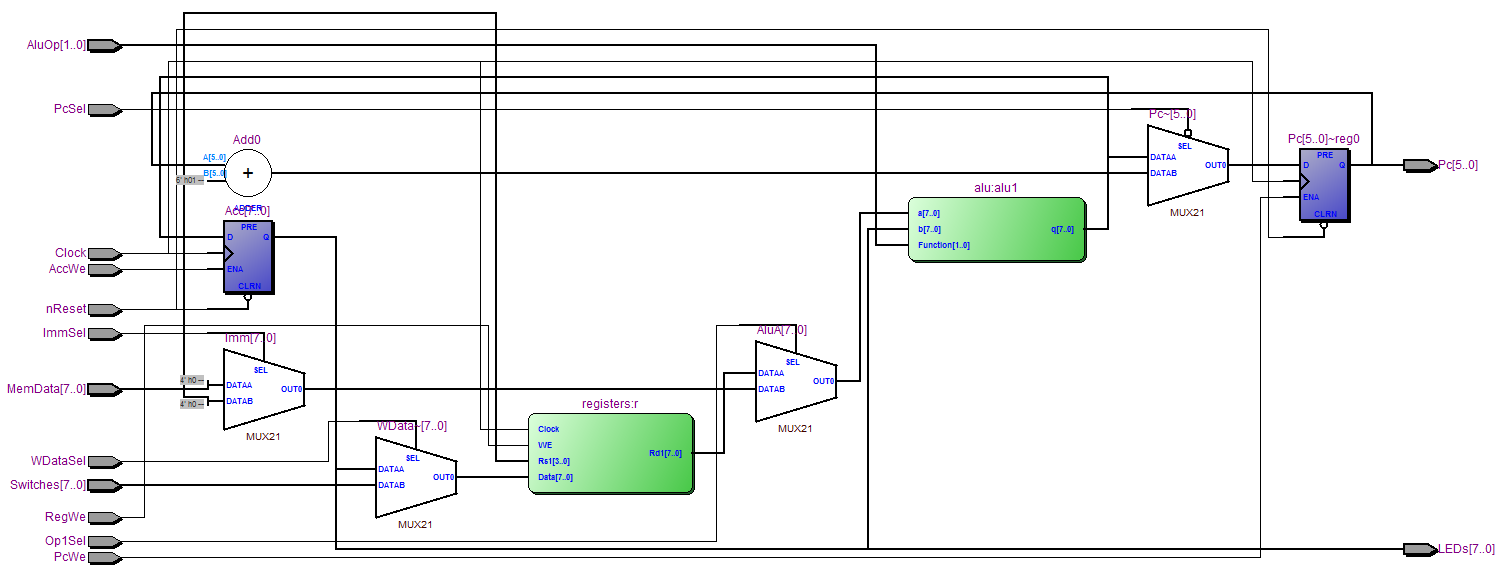
\includegraphics[width=\textwidth]{Figures/datapathsynth.png}
\caption{Synthesis of the Datapath}
\label{fig:datapathsynth}
\end{figure}


\section{CPU}
\subsection{Testbench}
%\todo[inline]{Describe testbench}

The testbench has two main parts; a task to commence the handshaking protocols, and a function to calculate the expected result. 
The handshaking task also contains assertions to verify the output. 
The function contains the constants and calculates the transform, with correct rounding.
The task can be seen in listing \ref{lstcputask} and the function is shown in listing \ref{lstcpufunction}.
These are used in a loop to test random sets of inputs. 
A few basic tests are also done with simple data. 

\lstinputlisting[firstline=31,style=sverilog,lastline=63,caption={Verification task to conduct the handshaking protocols. Assertions are used in this task to verify the output.},label=lstcputask]{../Implementation/cpu_stim.sv}
\lstinputlisting[style=sverilog,firstline=65, lastline=81,caption={Function used to calculate the expected output of the affine transform.},label=lstcpufunction]{../Implementation/cpu_stim.sv}




\subsection{Simulation Results}
%\todo[inline]{Full System Test}

Figure \ref{fig:cpusim} shows the output waveform of the test. 
Registers 0-5 contain the constants used. 
Registers 6 and 7 are used to store the initial $x_1$ and $y_1$ vector. 
Registers 9 and 10 are used to store the result and register 8 is used as a temporary register. 
The global error counter is shown, indicating that the whole system passes the test. 
Each iteration consists of a function call to calculate the expected outcome, and a task call to input the data. 
This process is then looped to test different datasets. 

\todo[inline]{Make a table of given inputs and expected outputs (real and rounded?)}

\begin{figure}
\includegraphics[height=\textheight-1cm]{Figures/cpusim.eps}
\caption{CPU simulation waveform}
\label{fig:cpusim}
\end{figure}

\subsection{Synthesis}
%\todo[inline]{Full system synthesis}

The top level module creates a instance of the controller, datapath and ROM. 
The interconnects are made here and the inputs and outputs to the controller are also made.
This top level synthesis is shown in figure~\ref{fig:cpusynth}.


\begin{figure}
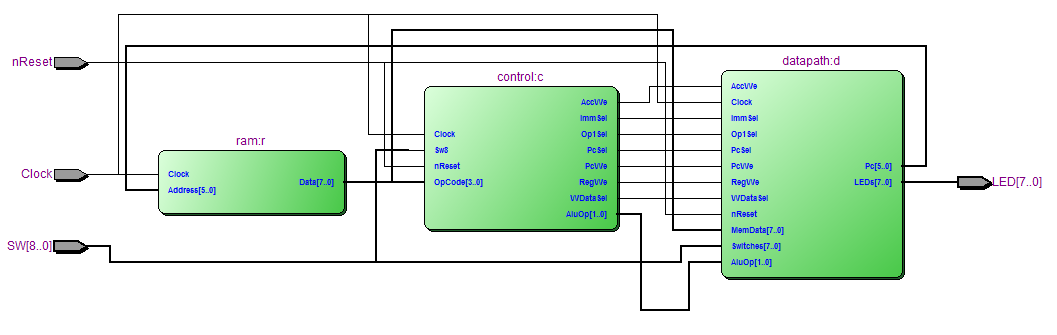
\includegraphics[width=\textwidth]{Figures/cpusynth.png}
\caption{Top level synthesis of the processor.}
\label{fig:cpusynth}
\end{figure}


%  DE0.tex
%  Document created by seblovett on seblovett-Ubuntu
%  Date created: Tue 01 Apr 2014 20:11:21 BST
%  <+Last Edited: Fri 04 Apr 2014 11:32:14 BST by hl13g10 on octopus +>

\section{DE0 Implementation}



%\todo[inline]{Use of the slow clock}
A counter was used to slow down the $50MHz$ clock supplied from the board. 
This slowed the processor down to a human usable speed.
The added logic from this is not included in the cost function.


%\todo[inline]{Demo define to allow for easier use during demo.}
To aid the demonstration, a small amount of extra logic is used to show if the opcode is a \texttt{WAIT} instruction. 
This can be turned on or off by used of a \textit{`define} statement declared in the \textit{options.sv} file.
It provides an insight in to the current state of the processor and if it is waiting for an input.

This is accomplished by the code seen in listing \ref{lstleds}.
The logic added by here is not included in the overall cost function and is added to aid the use. 


\lstinputlisting[style=sverilog, firstline=30, lastline=39,caption={Extra LED logic to show when the processor is executing a \texttt{WAIT} instruction.},frame=single,label=lstleds]{../Implementation/cpu.sv}

\todo[inline]{Issues encounterd}

Program Memory not allowing to be small. 



\todo[inline]{Synthesised logic. Put some sexy figures in here}



% Implementation

%  Conclusion.tex
%  Document created by seblovett on seblovett-Ubuntu
%  Date created: Tue 01 Apr 2014 20:11:41 BST
%  <+Last Edited: Wed 02 Apr 2014 13:32:59 BST by hl13g10 on octopus +>


\section{Conclusion}

Which objectives in intro have been done. 

Cost figure

General conclusion 

What I've learnt

Future work and improvements




\end{document}

